The composite AWP proposed in this work consists of a number of birefringent waveplates stacked at different azimuths relative to the optical axis. The set of characteristic dimensions of the waveplate together with the azimuthal angles therefore define a specific design. The characteristic dimensions of a waveplate is its thickness and stratification dimensions. In the first section of this chapter we present the Jones calculus which can be used to describe the polarization change of any non-depolarizing media such as birefringent waveplates. Subsequently we introduce and categorize waveplates in the context of the Jones calculus. The procedure of obtaining a design mainly consists of optimizing an objective function which is in turn based on the Jones calculus, which is described in the final section of this chapter.

\section{Jones calculus}
\label{sec:jonescalc}
The Jones calculus or specifically the Jones matrices can be used to describe the non-depolarizing polarimetric interaction of fully polarized light with matter. For that we first introduce a few general properties of the Jones matrices. In the following section we will then apply these properties to describe and categorize the different types of waveplates. Evidently, the following description of optical elements is only valid for changes with a linear relationship between the input and output amplitudes since it is based on a system of linear equations. Under these assumptions we can then express any transformation of an initial or input polarization state $\bm{\mathcal{E}}$ into another final output state $\bm{\mathcal{E}}'$ as:
\begin{equation}
    \bm{\mathcal{E}}' = \hat{T} \bm{\mathcal{E}},
\end{equation}
where $\hat{T}$ is the 2x2 complex Jones matrix specifying the interaction. With this many of the common operations defined in linear algebra can be reused and given a physical interpretation in the Jones calculus. For example the matrix product of two Jones matrices $\hat{T}_1$ and $\hat{T}_2$ represents a so called series or train of optical elements, where each matrix describes the polarimetric change caused by the respective element. This can be extended to multiple elements so that the final state in a train of $n$ consecutive elements is given by:
\begin{equation}
    \label{eq:jones_series_product}
    \bm{\mathcal{E}}' = \prod_{i=1}^{n} \hat{T}_i \bm{\mathcal{E}}.
\end{equation}
It is clear that since the product of two matrices does in general not commute the order of the factors is important \cite{Jones1941}. Therefore if $\hat{T}_1$ is the first element encountered by the light then the order of the indices has to be reversed. It is worth noting that in general the action of materials on the input state depends on the properties of the wave as well as how the interaction takes place. For example reflection from a surface depends on the incident angle or in case of waveplates the phase shift is proportional to the frequency. The Jones matrices themselves can therefore depend on a number of parameters reflecting the properties of the interaction, material and input state. Furthermore, since all Jones matrices are 2x2 complex matrices they can be factored into a product of three matrices using the singular value decomposition. This means we can express any Jones matrix $\hat{T}$ in the following form:
\begin{equation}
    \label{eq:jones_singular_value_decomposition}
    \hat{T} = \hat{T}_{R2}\diag{p_1, p_2}\hat{T}_{R1},
\end{equation}
where $\hat{T}_{R1}$ and $\hat{T}_{R2}$ are unitary\footnote{A complex square matrix $\hat{U}$ is unitary if $\hat{U} \hat{U}^\dagger=\hat{I}$ where $\hat{I}$ is the identity matrix} matrices and $\diag{p_1, p_2}$ is a diagonal matrix whose entries are the singular values of $\hat{T}$. The squares of $p_1$ and $p_2$ can be calculated directly using the following expressions:
\begin{equation}
    p_{1,2}^2 = \frac{1}{2}\left(\tr(\hat{T}\hat{T}^{\dagger}) \pm 
    \sqrt{\tr(\hat{T}\hat{T}^{\dagger})^2-4\det(\hat{T}\hat{T}^{\dagger})}\right),
\end{equation}
where $\tr$ is the matrix trace and the sign is respectively positive and negative for $p_1$ and $p_2$. The physical interpretation of these two values becomes evident if we consider the effect of the matrix $\diag{p_1, p_2}$ on an input state. Specifically, it simply scales the amplitudes of the state and with that also the intensity. Additionally, since the singular values are non-negative and real we can assume that $p_2\leq p_1$. Therefore, if the light is not amplified by the element in question then we get the following condition:
\begin{equation}
    \label{eq:passitivity_condition}
    p_1^2 \leq 1,
\end{equation}
which is also a defining property of Jones matrices. In other words a complex 2x2 matrix is a Jones matrix if equation \ref{eq:passitivity_condition} is satisfied \cite{Barakat1987}. Similar to Jones vectors the Jones matrices are defined up to an arbitrary phase factor $e^{i\phi}$, which means that two matrices $\hat{T}$ and $e^{i\phi}\hat{T}$ are equivalent in the sense that their respective final output states have equal intensities. A standard convention is therefore to assume that $\det \hat{T}$ is positive. Furthermore, the representation of a Jones matrix in another coordinate system follows directly from the coordinate transformation for Jones vectors given by equation \ref{eq:jones_vector_transformation}. Specifically, the transformation of a Jones matrix $\hat{T}$ in system XY to another representation $\hat{T}'$ in system X'Y' is given by:
\begin{equation}
    \label{eq:jones_matrix_transformation}
    \hat{T}' = \hat{Q}(\theta)\hat{T}\hat{Q}(-\theta).
\end{equation}
It is important to distinguish between frame rotations and rotations of the actual element. In the first case we rotate the axes and the second case can be understood as a rotation of the vector. Therefore, in the case of a rotation of the element around the Z-axis the signs of the rotation matrices in equation \ref{eq:jones_matrix_transformation} are inverted. It is worth noting that we only have to consider rotations since they are the only geometrical transformations that actually preserve the physically invariant quantities \cite{GilPerez2017}. Another interesting concept are singular states of polarization. Specifically, the singular value decomposition readily shows that for any Jones matrix there exists two pairwise orthonormal states $\tilde{\bm{\eta}}_1$ and $\tilde{\bm{\eta}}_2$ for which the orthogonality is preserved, in other words their respective output states $\bm{\eta}_1'$ and $\bm{\eta}_2'$ are mutually orthogonal. Furthermore, from the definition of the singular values the states $\tilde{\bm{\eta}}_1$ and $\tilde{\bm{\eta}}_2$ are orthonormal eigenvectors of the matrix $\sqrt{\hat{T}\hat{T}^{\dagger}}=\hat{T}_{R1}^{\dagger}\diag{p_1, p_2}\hat{T}_{R1}$ and are given explicitly by the columns of $\hat{T}^{\dagger}$. We can therefore express the singular states as:
\begin{equation}
    \bm{\eta}_1 = \hat{T}^{\dagger}_{R1}\begin{pmatrix} 1 \\ 0 \end{pmatrix}, \qquad
    \bm{\eta}_2 = \hat{T}^{\dagger}_{R1}\begin{pmatrix} 0 \\ 1 \end{pmatrix},
\end{equation}
and calculate the output states:
\begin{align}
\begin{split}
    \bm{\eta}'_1 &= \hat{T}\tilde{\bm{\eta}}_1 = 
    p_1\hat{T}_{R2}\hat{T}_{R1}\tilde{\bm{\eta}}_1 =
    p_1\hat{T}_{R2}\begin{pmatrix} 1 \\ 0 \end{pmatrix}, \\
    \bm{\eta}'_2 &= \hat{T}\tilde{\bm{\eta}}_2 = 
    p_2\hat{T}_{R2}\hat{T}_{R1}\tilde{\bm{\eta}}_2 =
    p_2\hat{T}_{R2}\begin{pmatrix} 0 \\ 1 \end{pmatrix}.
\end{split}
\end{align}
These expressions for the final states can then be used to calculate their respective intensities as:
\begin{equation}
    \bm{\eta}'^{\dagger}_1\bm{\eta}'_1=p_1^2, \qquad 
    \bm{\eta}'^{\dagger}_2\bm{\eta}'_2=p_2^2, \qquad 
    \bm{\eta}'^{\dagger}_1\bm{\eta}'_2=0.
\end{equation}
If we further define the transmittance as the ratio between the transmitted intensity and the incident intensity, then we see that the states $\bm{\eta}_1$ and $\bm{\eta}_2$ are exactly the states with the highest and lowest transmittance respectively. In other words, with respect to any other normalized output state, the states $\bm{\eta}'_1$ and $\bm{\eta}'_2$ are the output states with the highest and lowest intensities, respectively. The last property we will introduce before applying these to describe waveplates in the Jones calculus is the normality of Jones matrices. As we shall see later this property is important for the calculation of the retardance for a given Jones matrix. Additionally, Jones matrices can be separated into two categories depending on the mutual orthogonality of their eigenvectors $\bm{\mathcal{E}}_q$ and $\bm{\mathcal{E}}_r$. The eigenvectors which are also known as the eigenstates or eigenpolarizations of $\hat{T}$ can be interpreted by considering their defining equations:
\begin{equation}
    \hat{T}\bm{\mathcal{E}}_q = \lambda_q\bm{\mathcal{E}}_q, \qquad 
    \hat{T}\bm{\mathcal{E}}_r = \lambda_r\bm{\mathcal{E}}_r,
\end{equation}
where $\lambda_q = |\lambda_q|e^{i\delta_q}$ and $\lambda_r = |\lambda_r|e^{i\delta_r}$ are the associated complex eigenvalues. In other words, the application of $\hat{T}$ to the eigenstates only scales them by a complex number but leaves the polarization type unchanged. Hence if $\bm{\mathcal{E}}_q$ and $\bm{\mathcal{E}}_r$ are mutually orthogonal then the Jones matrix is said to be normal or homogeneous and nonnormal or inhomogeneous if they are nonorthogonal. We can therefore define the nonnormality or inhomogeneity parameter $\eta$ as follows:
\begin{equation}
    \eta=|\bm{\mathcal{E}}^{\dagger}_q \bm{\mathcal{E}}_r|.
\end{equation}
This means that the inhomogenity is zero if $\hat{T}$ is normal and one if the eigenvectors are parallel, where the latter is also known as the degenerate case. To calculate the inhomogeneity and verify that a given Jones matrix $\hat{T}$ is normal we use another derived expression for $\eta^2$ which is given by:
\begin{equation}
    \eta^2 = \frac{2||\hat{T}||_2^2-|\tr\hat{T}|^2-|(\tr\hat{T})^2-4\det\hat{T}|}{2||\hat{T}||_2^2-|\tr\hat{T}|^2+|(\tr\hat{T})^2-4\det\hat{T}|},
\end{equation}
where $||\hat{T}||_2=\sqrt{\tr \hat{T}^{\dagger} \hat{T}}$ denotes the Frobenius norm of $\hat{T}$ \cite{Lu1994}. With this we can introduce and categorize waveplates in the context of the Jones calculus which is shown in the following section. 

\section{Waveplates}
\label{sec:waveplates}
To explain how a waveplate works we assume that the materials are non-absorbing and neglect interface effects. These effects will be taken into consideration later on in the mathematical description. Additionally, to avoid refraction we always assume normal incidence of the light beam on the waveplate. In the case where we only consider birefringence the operation of a waveplate or retarder is fairly simple. One of the two polarization states of the wave is caused to have its phase evolve faster compared to the other state. Therefore, depending on the distance the wave travels in the waveplate, the amount one field component is lagging behind the other can be controlled. Using this principle it is in theory possible to convert any initial polarization state into any other state. This is shown in figure \ref{fig:waveplate_conversions}, where the positive values indicate that $E_y$ leads $E_x$ and similarly the negative values show that $E_y$ lags behind $E_x$ by the indicated amount. The waveplates in the context of this work consists of uniaxial materials i.e. they have a single optic axis. Therefore, if the $E_y$ component aligns with the fast axis, which is the axis with the lowest refractive index of the waveplate, then it is advanced compared to the $E_x$ component. Likewise, if the $E_y$ component is aligned with the slow axis of the waveplate then the $E_x$ component is advanced. Similarly, the slow axis is the axis or direction with the highest refractive index. The phase difference between two adjacent states in figure \ref{fig:waveplate_conversions} is $\frac{\pi}{4}$. Going clockwise this phase shift is subtracted and vice versa in the counterclockwise direction, so that eight steps make a full cycle. For example, if linearly polarized light is sent through a waveplate with its fast axis along the y-axis then the state will be shifted counterclockwise using the convention that $\delta=\delta_y-\delta_x$. This means that a phase shift of $-\frac{\pi}{2}$ causes \SI{45}{\degree} linear polarized light to emerge LCP and RCP for a phase shift of $+\frac{\pi}{2}$. Likewise, a phase shift of $\pm \pi$ causes the light to remain linearly polarized but with its plane of polarization rotated by \SI{90}{\degree}.

\begin{figure}[h]
    \centering
    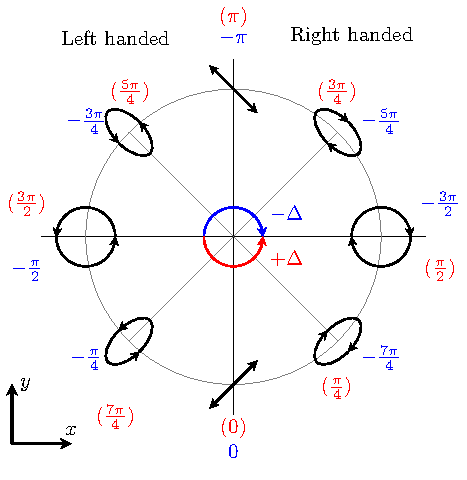
\includegraphics[scale=1.3]{images/theory/tikz_waveplate_conversions.pdf}
    \caption{The different polarization states when the y-component leads or lags behind the x-component by the indicated phase shifts $\pm \Delta$. Each step in the counterclockwise or clockwise direction subtracts or adds a phase shift of $\frac{\pi}{4}$ respectively.}
    \label{fig:waveplate_conversions}
\end{figure}

If we assume that the incident wave has components parallel and perpendicular to the optic axis of the waveplate, then two separate waves will propagate in the waveplate as we have seen in the previous chapter, that is the e- and o-wave. The phase speed of the e-wave is higher than that of the o-wave. Furthermore, if the incident light is parallel or perpendicular to the optic axis as in this case then we see no refraction of either of the waves, the final emerging wave will therefore be a superposition of the e- and o-wave. Additionally, due to the different phase velocities, the two waves will have a phase difference of $\Delta$ after passing through the waveplate. This phase difference is known as the retardance of the waveplate. For a waveplate of thickness $d$ the optical path difference is then given by:
\begin{equation}
    \Lambda = d|n_o - n_e|
\end{equation}
with $\Delta = k_0 \Lambda$ we therefore get the following expression for the phase difference:
\begin{equation}
    \label{eq:wp_eq}
    \Delta = \frac{2\pi}{\lambda_0}d|n_o - n_e|,
\end{equation}
where $\lambda_0$ is the wavelength of the wave in free space. There are three special types of waveplates: full, half and quarter waveplates. The full waveplate causes a phase shift of $2\pi$. That means the retardation is one wavelength or a full cycle in figure \ref{fig:waveplate_conversions}. The initial polarization state is therefore not altered. It is important to emphasize that this is only the case for monochromatic light. Since the materials in general are dispersive and because $\Delta$ directly varies as $\lambda_0^{-1}$. The condition that $\Delta = 2\pi$ or any other value can therefore only be fulfilled for monochromatic waves. This means in general that waveplates are chromatic which is the main problem with which we are concerned in this work. Full waveplates can therefore be used as narrow-wavelength filters if they are placed in between two crossed polarizers. Only the frequency component for which $\Delta$ is $2\pi$ will not have a component parallel to the final polarizer. 

A half waveplate causes a phase shift of $\pi$ between the e- and o-wave. Furthermore, we assume in the following that the initial polarization is linear and the plane of polarization is at some angle $\theta$ relative to the fast axis of the waveplate. As the name suggests, this phase shift causes one component to be delayed by half a wavelength relative to the other component. In the case of a positive uniaxial material this means that the e-wave is delayed by half a wave and the plane of polarization will be rotated by $2\theta$. An example of a half waveplate is shown in figure \ref{fig:half_waveplate}. In this example the material of the waveplate is positive uniaxial. Since then $n_o<n_e$ so that the e-wave is delayed relative to the o-wave. For a given wavelength and material it follows from equation \ref{eq:wp_eq} that $d$ must be equal to $\frac{1}{2}\frac{\lambda_0}{|n_o - n_e|}$. 

\begin{figure}[h]
    \centering
    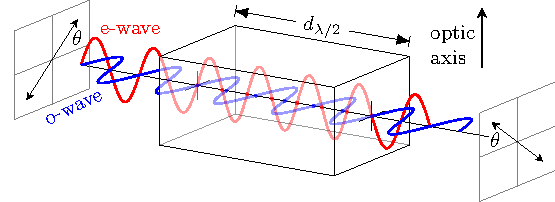
\includegraphics[scale=1.45]{images/theory/tikz_half_waveplate.pdf}
    \caption{A half waveplate consisting of a positive uniaxial material. The e-wave is delayed relative to the o-wave since it propagates slower. Adjusting the thickness $d_{\lambda/2}$ gives a final relative phase shift of $\pi$. This phase shift causes the polarization plane to be rotated by $2\theta$, where $\theta$ is the angle between the fast axis and the polarization plane of the waveplate. The dots along the axis of propagation indicate half a wavelength of the similar colored wave.}
    \label{fig:half_waveplate}
\end{figure}

As we saw earlier in figure \ref{fig:waveplate_conversions}, the polarization state is periodic with a periodicity of $2\pi$. It therefore follows from equation \ref{eq:wp_eq} that a waveplate with an additional thickness of $d_{\lambda}=\frac{\lambda_0}{|n_o - n_e|}$ still functions as a half waveplate. And with the same reasoning, an additional thickness of $md_{\lambda}$ (where $m$ is a whole number) does not change the final polarization state. The thickness of a half waveplate is therefore given by:

\begin{equation}
    \label{eq:thickness_half_waveplate}
    d_{\lambda/2} = \frac{(2m+1)\lambda_0}{2|n_o - n_e|}, \quad m=0,1,2,... 
\end{equation}

Furthermore, the effect that a half waveplate rotates the plane of polarization by $2\theta$ is also true for other elliptical polarization states. This is because a half waveplate always shifts one component by half a wave relative to the other component. Additionally, the handedness of the polarization state is inverted. We see this from figure \ref{fig:waveplate_conversions} where the effect of a half waveplate corresponds to half a rotation in the diagram. In other words, the final state is always on the opposite side of the initial state in the diagram. It is worth noting at this point, that linearly polarized light for which the polarization plane aligns with the slow or fast axis of any waveplate is unaffected by a waveplate, since in that case the light only has one component.

The final of the three special waveplate types is the quarter waveplate. Again, as the name suggests it shifts the relative phase by a quarter period or $\frac{\pi}{2}$. For linearly polarized light at an angle of \SI{45}{\degree} to either the slow or fast axis of a quarter waveplate, the light is converted into circular polarized light. An example of this setting is shown in figure \ref{fig:quarter_waveplate}.

\begin{figure}[H]
    \centering
    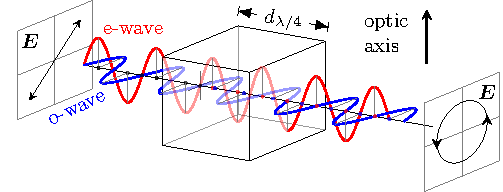
\includegraphics[scale=1.55]{images/theory/tikz_quarter_waveplate.pdf}
    \caption{\SI{45}{\degree} Linearly polarized light incident on a quarter waveplate consisting of a positive uniaxial material. In this case the slow axis is therefore along the optic axis. The thickness $d_{\lambda/4}$ is chosen so that the final phase difference between the e-wave and the o-wave is $\pi/2$. The final state is LCP since the material is positive uniaxial, for a negative uniaxial material it would be RCP. The colored dots indicate the accumulated phase difference.}
    \label{fig:quarter_waveplate}
\end{figure}

Because of the fact that the amplitudes of the components along the fast and slow axis initially are equal it follows that the final polarization state is circular. The same reasoning can be applied to circular light, which a quarter waveplate converts into linearly polarized light. Again, figure \ref{fig:waveplate_conversions} also gives an overview of some of the different possible conversions caused by a quarter waveplate. Specifically, a quarter waveplate shifts the polarization state a quarter cycle in the diagram. Similar to a half waveplate we get that the thickness $d_{\lambda/4}$ of a quarter waveplate is given by:

\begin{equation}
    \label{eq:thickness_quarter_waveplate}
    d_{\lambda/4} = \frac{(4m+1)\lambda_0}{4|n_o - n_e|}, \quad m=0,1,2,... 
\end{equation}

The number $m$ is known as the order of the waveplate. An order of $0$ means that it is the thinnest possible realization of a specific waveplate type. These waveplates are referred to as zero-order waveplates. Likewise, multiple-order waveplates have thicknesses that are a multiple of a full $2\pi$ phase shift plus the type specific phase shift. Evidently, for multiple-order waveplates $m$ is larger than zero. Waveplates are often multiple-order. For example a quartz quarter waveplate with a birefringence of $0.0092$ would have a thickness of only \SI{15}{\micro \meter} for a wavelength of \SI{550}{\nano \meter}. This makes it fragile as well as difficult to produce in contrast to a thicker multiple-order quarter waveplate. The half and quarter waveplates shown in figure \ref{fig:half_waveplate} and \ref{fig:quarter_waveplate} respectively, are examples of zero-order waveplates. The frequencies with which we are concerned in this work are in the higher GHz and the lower THz range. Consequently, already a zero-order quarter or half waveplate designed for these frequencies will have a thickness in the lower millimeter or centimeter range. A part of the problem is therefore to reduce the order of the designed waveplates, i.e. to keep them as thin as possible. This has to be taken into consideration since for higher orders the waveplates quickly become fairly thick which makes them impractical mainly due to high absorption losses \cite{Hecht}.

It is clear that it would quickly become complicated to predict the final polarization state of a polarized wave, after it has passed a series of waveplates and polarizers. Especially the way we have done it so far by considering polarization in terms of the individual field components. In the following section we will therefore introduce a better suited alternative method of describing the polarization and changes thereof. We will see that any polarization state can be described by a vector and each optical element by a matrix. This method reduces most calculations to matrix multiplications, which is especially useful for solving problems consisting of a series of optical elements.

\section{Jones calculus}
\label{sec:jones_calc}
% TODO_2 this section below
In the first section of this chapter we presented a phenomenological description of waveplates for which we assumed them to be fully transparent, i.e. the intensity of the incident light was equal to the intensity of the transmitted light. Under this assumption such ideal elements only exhibit birefringence and we will therefore refer to them as retarders or ideal waveplates. Furthermore, in the Jones calculus these ideal waveplates are represented by unitary matrices. Later in this section we will describe and add diattenuators to the framework. The diattenuator will allow us to quantify absorption by the waveplates and it especially simplifies the description of anisotropic absorption effects such as dichroism, reflection losses and transmission losses. In theory combined the retarder and diattenuator, known as a diattenuating retarder, constitute a complete model of the waveplate and even of any non-depolarizing material. In the following we classify and categorize retarders according to the polarization type of their eigenstates, consequently there are three different types of retarders; elliptic, circular and linear. 

\subsection{Retarders}
Similar to the different polarization types the most general type of retarder is the elliptic retarder which is characterized by the following eigenstates:
\begin{align}
\begin{split}
    \label{eq:ellip_pol_eigenstates}
    \bm{\mathcal{E}}_1(\alpha, \delta) &= 
    \begin{pmatrix} c_{\alpha} e^{-i\delta /2} \\ s_{\alpha} e^{i\delta /2} \end{pmatrix}
    = 
    \begin{pmatrix} c_{\chi} c_{\psi} - i s_{\chi} s_{\psi} \\ 
    c_{\chi} s_{\psi} + i s_{\chi} c_{\psi} \end{pmatrix},
    \\
    \bm{\mathcal{E}}_2 \left( \frac{\pi}{2} - \alpha, \delta+\pi \right) &= 
    \begin{pmatrix} -i s_{\alpha} e^{-i\delta /2} \\ i c_{\alpha} e^{i\delta /2} \end{pmatrix}
    = 
    \begin{pmatrix} -c_{\chi} s_{\psi} + i s_{\chi} c_{\psi} \\ 
    c_{\chi} c_{\psi} + i s_{\chi} s_{\psi} \end{pmatrix},
\end{split}
\end{align}
where we have set $\sin(x) = s_x$ and $\cos(x) = c_x$ which we use from here on. We see that $\bm{\mathcal{E}}_1$ and $\bm{\mathcal{E}}_2$ are both general elliptical polarization states, where the specific shape of their respective polarization ellipses is determined by the parameters $\alpha$ and $\delta$. It is worth emphasizing that $\delta$ is not the phase difference of the input state but a characterizing parameter of the retarder also known as the circularity. The corresponding Jones matrix $T_R(\alpha, \delta, \Delta)$ representing the elliptical retarder is given by:
\begin{equation}
    \hat{T}_R(\alpha, \delta, \Delta) = 
    \begin{pmatrix} 
    c^2_{\alpha}  e^{i\Delta /2} + s^2_{\alpha} e^{-i\Delta /2} & i s_{2\alpha} s_{\Delta/2} e^{-\delta} \\ 
    i s_{2\alpha} s_{\Delta/2} e^{-\delta} & s^2_{\alpha} e^{i\Delta/2} + c^2_{\alpha} e^{-i\Delta /2}
    \end{pmatrix}, 
\end{equation}
which introduces a phase difference of $\Delta$ between its eigenstates $\bm{\mathcal{E}}_1$ and $\bm{\mathcal{E}}_2$. In other words we can define the retardance $\Delta$ in terms of the arguments or phases of the eigenvalues as follows:
\begin{equation}
    \label{eq:jones_ret_def}
    \Delta = |\delta_r-\delta_q|.
\end{equation}
This is a reasonable definition if we consider the definition of the eigenstates and the polar form of the eigenvalues. That is the global phase change, which is also the only change, of each eigenstate is the phase of the eigenvalue. Especially, in the case of birefringent waveplates for which the linear eigenstates align with the fast and slow axis of the birefringent material we get exactly an additional phase shift of $\Delta$ between field components along said axes. Furthermore, we see that this is in fact the most general representation of a retarder, since the coefficients of any 2x2 unitary matrix can be factorized in this manner. If we change the frame in which we represent $\hat{T}_R(\alpha, \delta, \Delta)$ so that it aligns with the mayor and minor axes of the polarization ellipse of $\bm{\mathcal{E}}_1$, then $\psi=0$ for an orientation of \SI{0}{\degree} and therefore $\delta=\frac{\pi}{2}$, $\alpha=\chi$. With this the Jones matrix reduces to the following:
\begin{equation}
    \hat{T}_R\left(\chi, \frac{\pi}{2}, \Delta\right) = 
    \begin{pmatrix} 
    c^2_{\chi} e^{i\Delta /2} + s^2_{\chi} e^{-i\Delta /2} & s_{2\chi} s_{\Delta/2} \\
    -s_{2\chi} s_{\Delta/2} & s^2_{\chi} e^{i\Delta /2} + c^2_{\chi} e^{-i\Delta /2}
    \end{pmatrix}. 
\end{equation}

In the case of circular polarized eigenstates $\bm{\mathcal{E}}_1$ and $\bm{\mathcal{E}}_2$ the polarization ellipse reduces to a circle and $\chi=\frac{\pi}{4}$ so that $\delta=\frac{\pi}{2}$ and $\alpha=\frac{\pi}{4}$. A retarder with circular eigenstates is known as a circular retarder or rotator since in this case the Jones matrix takes on the following form:
\begin{equation}
    \hat{T}_{RC}(\Delta)=\hat{T}_R\left(\frac{\pi}{4}, \frac{\pi}{2}, \Delta\right) = 
    \begin{pmatrix} 
    c_{\Delta/2} & s_{\Delta/2} \\
    -s_{\Delta/2} & c_{\Delta/2}
    \end{pmatrix},
\end{equation}
which is also the representation of a rotation matrix $\hat{Q}(\theta)$ with $\theta=\Delta/2$. In other words the effect of $\hat{T}_{RC}(\Delta)$ is equal to a rotation of the principal axes of an incident state by $\theta=\Delta/2$. The final type is the linear retarder which is characterized by having linear eigenstates. For this type $\chi=0$, therefore $\delta=0$ and $\alpha=\psi$. With this the Jones matrix of the linear retarder is given by:
\begin{equation}
    \hat{T}_{RL}\left(\psi, \Delta\right) = 
    \begin{pmatrix} 
    c^2_{\psi} e^{i\Delta /2} + s^2_{\psi} e^{-i\Delta /2} & is_{2\psi} s_{\Delta/2} \\
    is_{2\psi} s_{\Delta/2} & s^2_{\psi} e^{i\Delta /2} + c^2_{\psi} e^{-i\Delta /2}
    \end{pmatrix},
\end{equation}
and if we again align the coordinate frame with the mayor and minor axes of its eigenstates then $\psi=0$ and $\hat{T}_{RL}$ adopts the following diagonal form:
\begin{equation}
    \hat{T}_{RL}\left(\psi=0, \Delta\right) \equiv \hat{T}_{RL0}\left(\Delta\right) = 
    \begin{pmatrix} 
    e^{i\Delta /2} & 0 \\
    0 & e^{-i\Delta /2}
    \end{pmatrix},
\end{equation}
which is known as a horizontal linear retarder. In this frame we directly recognize the total phase shift $\Delta$ of the eigenstates. Furthermore, we see that the mayor and minor axis of the polarization ellipse of the eigenstates align with the fast and slow axis of the retarder. If we set $\Delta=\pi$ in the expression for the linear retarder we get the Jones matrix for the half wave retarder or transparent half waveplate as follows:
\begin{equation}
    \hat{T}_{RL}(\psi, \pi)= 
    \begin{pmatrix} 
    c_{2\psi} & s_{2\psi} \\
    s_{2\psi} & -c_{2\psi}
    \end{pmatrix}.
\end{equation}
We see that $\hat{T}_{RL}(\psi, \pi)$ is equivalent to a rotation by $-2\psi$ and an inversion of the y-component where the latter can be represented by $\hat{T}_{RL}(0, \pi)$. Therefore, essentially $\hat{T}_{RL}(\psi, \pi)$ inverts the handedness and then rotates the polarization ellipse of the state by $-2\psi$. These two actions combined are also known as an improper rotation. A circular polarized state therefore remains circular but has its handedness reversed by the action of $\hat{T}_{RL}(\psi, \pi)$. Finally, we can also see this by writing $\hat{T}_{RL}(\psi, \pi)$ to obtain the following representation of the Jones matrix describing the half wave retarder:
\begin{equation}
    \label{eq:l2_wp_effect}
    \hat{T}_{RL}(\psi, \pi)\equiv
    \hat{T}_{1/2}(\psi)=
    \hat{Q}(-2\psi)\hat{T}_{RL}(0, \pi)=\hat{Q}(-2\psi)\diag{1,-1}.
\end{equation}
If the input light is for example linear horizontal polarized and $\psi=\frac{\pi}{4}$ then the inversion leaves the state unaffected but the rotation produces an output state which is linear vertical polarized.
Similarly, if we set $\Delta=\pi/2$ then the expression for the linear retarder reduces to the following:
\begin{align}
\begin{split}
    \hat{T}_{1/4}(\psi)\equiv\hat{T}_{RL}(\psi, \pi/2)
    &=\frac{1}{\sqrt{2}}\left(\hat{I}+i\hat{Q}(-2\psi)\hat{T}_{RL}(\pi, \pi)\right)
    \\
    &=\frac{1}{\sqrt{2}}\left(\hat{I}+i\hat{T}_{1/2}(\psi)\right),
\end{split}
\end{align}
which is the Jones matrix for a quarter wave retarder. This expression shows that $\hat{T}_{RL}(\psi, \pi/2)$ is equivalent to the effect of $\hat{T}_{1/2}(\psi)$ followed by a \SI{90}{\degree} phase shift this new state is then superimposed on the input state. For example a linear horizontal state is first transformed into a linear vertical polarized state and then shifted by a quarter period. This rotated and shifted state is then further superimposed on the horizontal input state so that the output state will be RCP. 

It is in fact possible to represent any linear retarder using a combination of rotation matrices $\hat{Q}$ and horizontal linear retarders $\hat{T}_{RL0}$ as follows:
\begin{equation}
    \hat{T}_{RL}(\psi, \Delta)=\hat{T}_{RC}(-2\psi)\hat{T}_{RL0}(\Delta)\hat{T}_{RC}(2\psi)=
    \hat{Q}(-\psi)\hat{T}_{RL0}(\Delta)\hat{Q}(\psi).
\end{equation}
In other words a linear retarder is equivalent to a horizontal linear retarder $\hat{T}_{RL0}(\Delta)$ placed between a left- and right-handed circular retarder $\hat{T}_{RC}(-2\psi)$ and $\hat{T}_{RC}(2\psi)$ respectively. In general an elliptic retarder $\hat{T}_R(\alpha, \delta, \Delta)$ can be realized by the following combination of elements \cite{GilPerez2017}:
\begin{equation}
    \hat{T}_R(\alpha, \delta, \Delta)=
    \hat{T}_{RL0}(-\delta)\hat{Q}(-\alpha)\hat{T}_{RL0}(\Delta)\hat{Q}(\alpha)\hat{T}_{RL0}(\delta).
\end{equation}

\subsection{Diattenuators}
In the following we will introduce the diattenuator in a similar fashion as we did with the retarder. It is used to describe the polarization dependent transmittance of the waveplate. Any element for which the singular values $p_1$ and $p_2$ of its Jones matrix are mutually different can be considered a diattenuator \cite{Savenkov2005}. This means that for example matrices $\hat{T}_r$ and $\hat{T}_t$ describing the transmission and reflection at an interface are examples of Jones matrices representing diattenuators. If we further consider homogeneous diattenuators then we can again use a singular value decomposition as in equation \ref{eq:jones_singular_value_decomposition} to factorize the diattenuator Jones matrix as follows:
\begin{equation}
    \label{eq:diattenuator_singular_value_decomposition}
    \hat{T}_D = \hat{T}_D^{\dagger} = \hat{T}_R\hat{T}_{DL0}\hat{T}_R^{\dagger}, 
    \qquad 
    \hat{T}_{DL0}=\diag{p_1, p_2}.
\end{equation}
We know from the previous section that $p_1^2$ and $p_2^2$ are respectively the maximum and minimum transmittance. We can therefore use $p_1$ and $p_2$ to define the diattenuation in the Jones calculus as follows: 
\begin{equation}
    \label{eq:diattenuation_1}
    D = \frac{p_1^2-p_2^2}{p_1^2+p_2^2}
\end{equation}
Furthermore, as with the retarders the diattenuators are also grouped or categorized based on the polarization type of their associated eigenstates. This means that the most general type of homogeneous diattenuators is the elliptic diattenuator with eigenstates given in equation \ref{eq:ellip_pol_eigenstates}. Additionally, equation \ref{eq:diattenuator_singular_value_decomposition} shows that the diattenuator is represented by a Hermitian\footnote{A complex square matrix $\hat{H}$ is Hermitian if $\hat{H}=\hat{H}^{\dagger}$.} matrix. This means that the Jones matrix of the most common or general diattenuator can be written as:
\begin{equation}
    \hat{T}_D(\alpha, \delta, p_1, p_2) = 
    \begin{pmatrix} 
    p_1 c_{\alpha}^2 + p_2 s_{\alpha}^2 & s_{\alpha}c_{\alpha}(p_1-p_2)e^{-i\delta} \\
    s_{\alpha}c_{\alpha}(p_1-p_2)e^{i\delta} & p_1 s_{\alpha}^2 + p_2 c_{\alpha}^2
    \end{pmatrix},
\end{equation}
for which we assume that $0\leq p_2\leq p_1$. If $p_2=0$ then $\hat{T}_D(\alpha, \delta, p_1, 0)$ represents a total elliptic polarizer which completely absorbs the $\bm{\mathcal{E}}_2$ eigenstate. If we align the axes of the frame in which $\hat{T}_D(\alpha, \delta, p_1, p_2)$ is represented to the axes of the polarization ellipse of $\bm{\mathcal{E}}_1$ as in the case of the horizontal retarders, then we get the so called horizontal elliptic diattenuator. Again $\psi=0$ so that $\delta=\frac{\pi}{2}$, $\alpha=\chi$ which in $\hat{T}_D(\alpha=\chi, \delta=\frac{\pi}{2}, p_1, p_2)$ yields the respective Jones matrix representing the horizontal elliptic diattenuator. Figure \ref{fig:horizontal_diattenuator} shows a horizontal diattenuator and the effect of the diattenuation on its elliptical eigenstates. We see that in general the diattenuator changes the shape of the polarization ellipse depending on $p_1$ and $p_2$, while in contrast the retarders only rotate or change the handedness of the ellipse. This is also underlined by the fact that $\det(\hat{T}_D) = p_1p_2 \leq 1$ while $\det(\hat{T}_{R}) = 1$.

\begin{figure}[h]
    \centering
    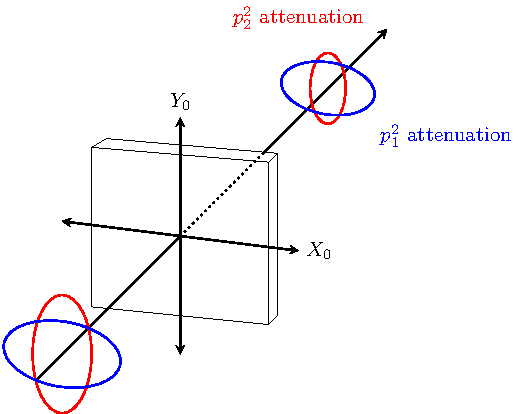
\includegraphics[scale=1]{images/theory/tikz_horizontal_diattenuator.pdf}
    \caption{Elliptical diattenuator at an angle of \SI{0}{\degree} to its intrinsic frame also known as a horizontal diattenuator. In this case the axes of the diattenuator align with the mayor and minor axis of its eigenstates so that the two eigenstates $\bm{\mathcal{E}}_1$, $\bm{\mathcal{E}}_2$ directly experience an intensity attenuation of respectively $p_1^2$ and $p_2^2$.}
    \label{fig:horizontal_diattenuator}
\end{figure}

A diattenuator which is characterized by circular eigenstates, so that $\chi=\frac{\pi}{4}$ and therefore $\delta=\frac{\pi}{2}$, $\alpha=\frac{\pi}{4}$, is represented by the following Jones matrix:
\begin{equation}
    \hat{T}_{DC}(p_1, p_2) = \hat{T}_D\left(\frac{\pi}{4}, \frac{\pi}{2}, p_1, p_2\right) =
    \frac{1}{2}
    \begin{pmatrix} 
    p_1 + p_2 & -i(p_1 - p_2) \\
    i(p_1 - p_2) & p_1 + p_2
    \end{pmatrix}.
\end{equation}
It is worth noting that for $p_2=0$ $\hat{T}_{DC}(p_1, p_2=0)$ represents a circular polarizer which completely extinguishes the circular eigenstate $\bm{\mathcal{E}}_2$. The final of the three types is the linear diattenuator. In this particular case the eigenstates are linearly polarized so that $\chi=0$ and therefore $\delta=0$, $\alpha=\psi$. The linear diattenuator can accordingly be represented by the following Jones matrix:
\begin{equation}
    \hat{T}_{DL}(\psi, p_1, p_2) = 
    \begin{pmatrix} 
    p_1c_{\psi}^2 + p_2s_{\psi}^2 & c_{\psi}s_{\psi}(p_1 - p_2) \\
    c_{\psi}s_{\psi}(p_1 - p_2) & p_1s_{\psi}^2 + p_2c_{\psi}^2
    \end{pmatrix},
\end{equation}
which for $p_2=0$ represents the well known linear polarizer realized by for example a wiregrid polarizer. The Jones matrix then takes on the form:
\begin{equation}
    \hat{T}_{DL}(\psi, p_1, 0) = \hat{T}_{D}(\psi, 0, p_1, 0) =
    p_1
    \begin{pmatrix} 
    c_{\psi}^2 & c_{\psi}s_{\psi} \\
    c_{\psi}s_{\psi} & s_{\psi}^2
    \end{pmatrix}.
\end{equation}
It is worth noting that Malus' law can easily be derived from this, if we consider horizontally polarized light with an initial intensity $I_0=|E_x|^2$, as follows:
\begin{equation}
    \bm{\mathcal{E}}_{\SI{0}{\degree}}^{\dagger}
    \hat{T}_{DL}(\psi, p_1=1, 0)\bm{\mathcal{E}}_{\SI{0}{\degree}} = |E_x|^2p_1^2c_{\psi}^2 = I_0 c_{\psi}^2.
\end{equation}

Furthermore, oriented at \SI{0}{\degree} the horizontal diattenuator takes on the diagonal form $\hat{T}_{DL0}(p_1, p_2) = \hat{T}_{DL}(0, p_1, p_2)=\hat{T}_{D}(0,0,p_1,p_2)=\diag{p_1, p_2}$ and $\diag{p_1, 0}$ for a linear polarizer at $\psi = \SI{0}{\degree}$. Similar to the general form of the retarder, the elliptic diattenuator can also be written as a product of rotation matrices, horizontal retarders and diattenuators as follows:
\begin{align}
\begin{split}
    \hat{T}_{D}(\alpha, \delta, p_1, p_2) 
    &= \hat{T}_{RL0}(-\delta)\hat{T}_{DL}(\alpha, p_1, p_2)\hat{T}_{RL0}(\delta) \\
    &= \hat{T}_{RL0}(-\delta)\hat{Q}(-\alpha)\hat{T}_{DL0}(p_1, p_2)\hat{Q}(\alpha)\hat{T}_{RL0}(\delta).
\end{split}
\end{align}
This means that any diattenuator is equivalent to a linear diattenuator placed between two crossed linear retarders \cite{Gil2016}. 

\subsection{Diattenuating retarders - waveplates}
With the introduction of the diattenuator we can finally describe real linear retarders or specifically waveplates which in general show some amount of diattenuating effects \cite{D.CLARKE1971}. For this purpose we can assume that the optic axes of the retarder and diattenuator coincide, this assumption can be shown to be equivalent to the normality condition \cite{Bass1995}. Furthermore, we know from the previous section that states polarized along the fast or slow axis of the birefringent material of the waveplate will not undergo a polarization change as it passes through the waveplate. The eigenstates of a birefringent material are therefore linear and the planes of polarization coincide with the slow and fast axes of the material. Consequently, we can describe the waveplate using a linear retarder and diattenuator. A linear nonideal retarder or diattenuating retarder can be represented by the Jones matrix $\hat{T}_{RDL}$, which depends on four parameters; the orientation angle $\psi$ between the fast axis of the retarder $X_0$ and the axis $X$ of the reference frame, the principal intensities $p_1^2$ and $p_2^2$ and finally on the retardance $\Delta$. This means that $\hat{T}_{RDL}$ can be represented by the following product of matrices:
\begin{equation}
    \hat{T}_{RDL}(\psi, \Delta, p_1, p_2) = \hat{Q}(-\psi)\hat{T}_{RL0}(\Delta)\hat{T}_{DL0}(p_1, p_2)\hat{Q}(\psi),
\end{equation}
we can carry out the multiplication to obtain the following representation of $\hat{T}_{RDL}$:
\begin{equation}
    \hat{T}_{RDL}(\psi, \Delta, p_1, p_2) = 
    \begin{pmatrix} 
    p_1e^{i\Delta/2}c_{\psi}^2+p_2e^{-i\Delta/2}s_{\psi}^2 & c_{\psi}s_{\psi}\left(p_1e^{i\Delta/2}-p_2e^{-i\Delta/2}\right) \\
    c_{\psi}s_{\psi}\left(p_1e^{i\Delta/2}-p_2e^{-i\Delta/2}\right) & 
    p_1e^{i\Delta/2}s_{\psi}^2+p_2e^{-i\Delta/2}c_{\psi}^2
    \end{pmatrix}.
\end{equation}
This Jones matrix describes a single waveplate and a train of waveplates is then simply given by the product of the individual $\hat{T}_{RDL}$ matrices. Obtaining the retardance and diattenuation of the final product can be achieved with a polar decomposition, which states that for any complex 2x2 matrix $\hat{T}$ there exist positive-definite\footnote{A Hermitian matrix $\hat{H}$ is positive-definite if $\bm{\mathcal{E}}^{\dagger}\hat{H}\bm{\mathcal{E}}$ is positive for any $\bm{\mathcal{E}}$} Hermitian matrices $\hat{H}$ and $\hat{H}'$ and a unitary matrix $\hat{U}$ such that $\hat{T}=\hat{U}\hat{H}=\hat{H}'\hat{U}$. This means that an arbitrary Jones matrix describing any non-depolarizing optical element can be written as a product of a retarder and diattenuator as follows \cite{GilPerez2017}:
\begin{equation}
    \hat{T} = \hat{T}_R\hat{T}_D = \hat{T}_D'\hat{T}_R.
    \label{eq:diattenuation_retarder}
\end{equation}
Furthermore, the retardance $\Delta$ defined through the eigenvalues of $\hat{T}_R$ can be calculated using the following expression:
\begin{equation}
    \Delta = 2 \cos^{-1} \frac{\left|\tr\hat{T}+\frac{\det \hat{T}}{\left|\det \hat{T}\right|} \tr \hat{T}^{\dagger}\right|}{2\sqrt{\tr \hat{T}\hat{T}^{\dagger}+2\left|\det \hat{T}\right|}},
\end{equation}
which follows from the calculation of the eigenvalues of $\hat{T}$. We have to assume that the transmittances $p_1$ and $p_2$ are not zero since then $\hat{T}$ represents a polarizer for which the determinant of the corresponding Jones matrix is zero. Additionally, this equation is only valid for homogeneous Jones matrices. In the inhomogeneous case the following expression has to be used instead:
\begin{align}
\begin{split}
    \label{eq:retardation_inhomogeneous}
    \Delta &= 2\cos^{-1}\left\{r\left[\frac{(1-\eta^2)(|\lambda_q|+|\lambda_r|)^2}
    {(|\lambda_q|+|\lambda_r|)^2-\eta^2(2|\lambda_q||\lambda_r|+\lambda_q^*\lambda_r+\lambda_q\lambda_r^*)}\right]^{1/2}\right\}, \\
    r &= \left|\cos \frac{\delta_q-\delta_r}{2}\right|
\end{split}
\end{align}
where $\lambda_{r,q}=|\lambda_{q,r}|e^{i\delta_{q,r}}$ are the eigenvalues of $\hat{T}$.
Similarly, the diattenuation $D$ can be calculated from the Jones matrix as follows:
\begin{equation}
    \label{eq:diattenuation_2}
    D=\sqrt{1-\frac{4|\det \hat{T}|^2}{(\tr \hat{T}\hat{T}^{\dagger})^2}},
\end{equation}
which has the advantage that it does not depend directly on $p_1$ and $p_2$. Again, in the case of an inhomogeneous Jones matrix equation \ref{eq:diattenuation_2} is invalid and the following equation should be used:
\begin{equation}
    \label{eq:diattenuation_inhomogeneous}
    D=\sqrt{1- \frac{4(1-\eta^2)^2|\lambda_q|^2|\lambda_r|^2}
    {\left(|\lambda_q|^2+|\lambda_r|^2-\eta^2(\lambda_q\lambda_r^*+\lambda_r\lambda_q^*)\right)^2}}.
\end{equation}
Expressions \ref{eq:retardation_inhomogeneous} and \ref{eq:diattenuation_inhomogeneous} are valid for $\eta \neq 0$ but evidently less efficient \cite{Lu1994}. With this we can describe a train of waveplates and subsequently characterize the final Jones matrix through the equivalent retardance and diattenuation. In the following section we will consider the wavelength dependency of waveplates and introduce the achromatic waveplate (AWP), which ideally has the special property of being wavelength independent. 

\section{Achromatic waveplates}
\label{sec:achromatic_waveplates}

As we have seen already waveplates are highly wavelength sensitive due to the inverse wavelength dependency of the phase shift but also due to dispersion of the refractive index and consequently dispersion of the birefringence. In other words the three parameters $\Delta$, $p_1$ and $p_2$ of the four parameters in total which characterize a linear diattenuating retarder or waveplate are wavelength dependent. There are several types of AWPs based on different techniques which can in theory compensate for this wavelength dependency. One possibility is to use the phase shift induced by total internal reflection which can be realized through a Fresnel Rhomb. Using this method it is possible to create an almost perfect AWP. The Fresnel Rhomb works over a large frequency range since the variation of retardance is solely due to dispersion causing the reflectance to become wavelength dependent \cite{Hecht}. They often cause strong spatial shifts of the light, take up more space and are hard to align since the retardation strongly depends on the angle. Another method is to combine waveplates of different materials. The problem with this method is that only the dispersion of the materials is compensated for and so the resulting range is relatively low \cite{Masson2006}. The AWPs presented in this work are based on a similar design principle as the THz achromatic quartz quarter waveplates (TAQ) developed by Masson and Gallot in \cite{Masson2006}. The TAQ is ultimately based on the work by Destriau and Prouteau in 1949 \cite{Destriau1949} where they showed that the serial combination of a half waveplate and a quarter waveplate for which $\psi=\SI{60}{\degree}$ results in a new achromatic quarter waveplate. This new AWP showed a $\frac{\pi}{2}$ phase shift over the whole visible range. Masson and Gallot extended this idea to the THz range by combining six quartz plates with variable thicknesses and again at different azimuths $\psi$. This higher number of plates was necessary due to the increased bandwidth of short THz pulses. The operational principle of this type of AWP is based on the partial cancellation each plate is causing with respect to the frequency. Each quartz waveplate was assumed to have a negligible dichroism. It was reported that at \SI{1}{\tera \hertz} crystalline quartz showed an ordinary and extraordinary refractive index of $n_o=2.108$ and $n_o=2.156$ respectively. Due to this low birefringence the total thickness of the TAQ is relatively large. Assuming isotropic absorption of the plates, the AWP can be described by the following product:
\begin{equation}
    \hat{T}_{M} = \prod_{i=1}^{n=6} \hat{T}_{RL}(\psi_i, \Delta_i) = 
    \begin{pmatrix} 
    A & B \\
    -B^* & A^*
    \end{pmatrix},
    \label{eq:equiv_matrix}
\end{equation}
where according to equation \ref{eq:wp_eq} the $\Delta_i$ are proportional to the frequency and the thickness $d_i$ of the i-th waveplate. From the previous section we know that $\hat{T}_M$ can be written as the product of a diattenuator and a retarder. Therefore, setting $p_1=p_2=1$ and comparing the coefficients of $\hat{T}_{M}$ to a retarder represented by $\hat{T}_{RL}(\psi, \Delta_M)$ they get an expression for the so called resulting retardation dephasing $\Delta_M$:
\begin{equation}
    \label{eq:retardation_dephasing}
    \tan^2 \frac{\Delta_M}{2} = \frac{\operatorname{Im}A^2+\operatorname{Im}B^2}
    {\operatorname{Re}A^2+\operatorname{Re}B^2}.
\end{equation}
It is worth noting that the value $\Delta_M$ is not the same as the retardance defined in equation $\ref{eq:jones_ret_def}$. Nevertheless, it can be understood as the phase shift induced by a linear retarder $\hat{T}_{RL}(\SI{45}{\degree}, \Delta_M)$ on a horizontal state. The problem of determining the parameters $\psi_i$ and $d_i$ to get the appropriate phase shift at each frequency can be formulated as an optimization problem where the objective is to minimize the following error function:
\begin{equation}
    \label{eq:mass_loss}
    L(\psi_i, d_i)_M=\sum_{\nu}\left(\Delta_M(\nu)-\frac{\pi}{2}\right)^2.
\end{equation}
They minimize $L(\psi_i, d_i)_M$ using a simulated annealing algorithm over the frequency range \SIrange{0.2}{2}{\tera \hertz} and their result is shown in table \ref{tab:masson_result}. For this set of parameters it is reported that the deviation of $\Delta_M$ from $\frac{\pi}{2}$ is less than \SI{3}{\percent} over the frequency range \SIrange{0.25}{1.75}{\tera \hertz} and that the total thickness of the TAQ is \SI{31.4}{\milli \meter}. 

\begin{table}[h]
    \centering
    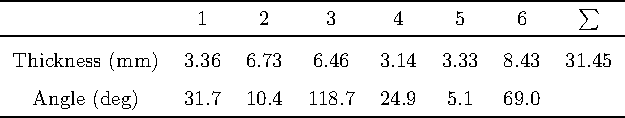
\includegraphics[scale=1]{images/theory/masson_result_table.pdf}
    \caption{Optimization result obtained by Masson and Gallot in \cite{Masson2006}. This particular TAQ consists of six plates of varying thicknesses and orientation angles.}
    \label{tab:masson_result}
\end{table}

A similar AWP is presented in another work by Wu, et al. Here they use sapphire instead of crystalline quartz which reduces the overall thickness of the AWP to \SI{2.453}{\milli \meter} since compared to quarts sapphire has a higher birefringence. They report a value of 3.39 and 3.07 for the ordinary and extraordinary refractive index respectively. Similarly, they optimize the loss function given in equation \ref{eq:mass_loss} and by stacking even up to 20 individual plates they obtain a deviation less than \SI{0.5}{\percent} from the $\pi/2$ target over the frequency range \SIrange{0.2}{2.0}{\tera \hertz}. Table \ref{tab:wu_result} shows their obtained values for the result with an overall thickness of \SI{2.453}{\milli \meter} consisting of six plates. This design was produced and characterized but showed more than a threefold increase in phase deviation compared to the optimization result. This deviation was attributed to angle misalignment and a mismatch between the used values from the actual values of the index of refraction of sapphire \cite{Wu2020}. 

\begin{table}[h]
    \centering
    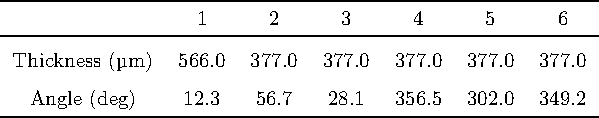
\includegraphics{images/theory/wu_result_table.pdf}
    \caption{Obtained parameters for $n=6$ published in \cite{Wu2020} with a design similar to that of Masson and Gallot. The higher birefringence of sapphire compared to quartz allows the plates to be thinner compared to the result by Masson and Gallot.}
    \label{tab:wu_result}
\end{table}

A possible reduction of the angle misalignment can in theory be achieved using selective laser-induced etching (SLE) to produce form birefringent waveplates. Simply put SLE is a two step process; first transparent fused silica glass is selectively modified using a laser and subsequently the volume connected to the surface of the structure is removed by wet chemical etching. This means that SLE allows the fabrication of 3D structures with a precision of around \SI{1}{\micro \meter} \cite{Hermans2014}. This technique has the potential of removing the alignment step in the assembly of the AWP by fabricating the structure from a single glass piece and thereby reducing angle alignment errors. Ornik et al. showed in \cite{Ornik2018} that it is possible to fabricate high quality form birefringent $\lambda/2$ THz waveplates using this technique. The waveplates have the same periodically stratified structure as the media discussed at the end of section \ref{sec:wave_prop}. Each plate is manufactured from a rectangular slab of fused silica glass using SLE. The plates consist of a series of glass bars separated by air grooves. The structure is homogeneous along the direction of propagation, in other words the plates are stratified throughout the thickness $d_i$. In total four waveplates were characterized with different air and glass layer thicknesses as well as different plate thicknesses. One of the four plates is shown in figure \ref{fig:SLE_waveplate_JO_} next to a one euro coin.

\begin{figure}
    \centering
    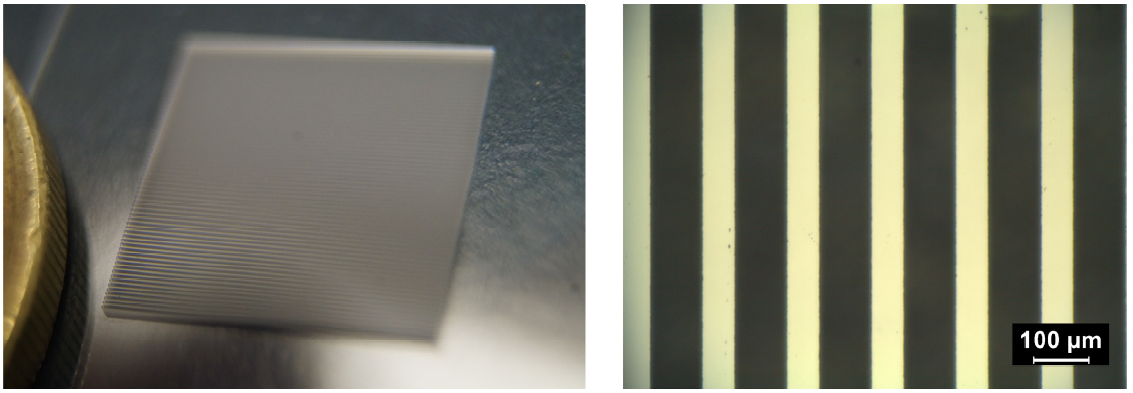
\includegraphics[scale=0.45]{images/theory/SLE_waveplate_JO_.png}
    \caption{Left figure shows one of the four characterized fused silica glass waveplates next to a one euro coin. Right figure shows a microscope image of the same plate. The bright stripes are the glass bars while the black are air gaps. Source: \cite{Ornik2018}}
    \label{fig:SLE_waveplate_JO_}
\end{figure}

Among other characterizing measurements the transmitted intensity was measured after passing a linear polarizer for different azimuths $\psi$. We know from equation \ref{eq:l2_wp_effect} that the effect of a $\lambda/2$ retarder is to rotate the mayor axes of the polarization ellipse by $-2\psi$. Therefore, if the input state is $\bm{\mathcal{E}}_{\SI{45}{\degree}}$ we expect a minimum in the transmitted intensity since then the output state is perpendicular to the transmission axis of the polarizer. This is of course only true for the frequencies where the retardance of the plate is $\pi$. In fact, if we assume the polar decomposition of the waveplate is a linear diattenuating retarder then we can show\footnote{See section \ref{sec:transmission_min} of the appendix} the following equation for the azimuth of the minimum transmittance:  
\begin{equation}
    \psi_{min}=\arctan\left(\sqrt{\frac{p_2}{p_1}}\right)
\end{equation}
Therefore, only if $p_1=p_2$ do we get the minimum transmittance at an azimuth of \SI{45}{\degree}. Although measurements of the intensity at different azimuths showed that the minimum transmission is not obtained for $\psi=\SI{45}{\degree}$ but rather at \SI{46}{\degree}, \SI{46}{\degree}, \SI{47}{\degree}, \SI{49}{\degree} for increasing thickness of the four waveplates. This means that in the case of form birefringent fused silica glass waveplates and waveplates consisting of anisotropic materials dichroism should be taken into consideration. In turn, this furthermore means that we cannot simply rely on optimizing the retardance to obtain designs which produce pure output polarizations. Building onto the method of Masson and Wu we therefore need to implement new loss or objective functions for the $\lambda/4$ and $\lambda/2$ waveplate types if we want to take dichroism into account. At the same time the form birefringent AWP type allows us to directly optimize the birefringence of each individual plate, but it also comes with the cost of adding $2n$ more dimensions to the optimization problem. To summarize, the proposed AWP design consists of $n$ individual form birefringent plates where each plate has a similar structure as the one shown in figure \ref{fig:SLE_waveplate_JO_}. Similar to the TAQ waveplate, each individual plate is oriented at an azimuthal angle $\psi_i$ relative to the mayor axes of the polarization ellipse of the initial input state. Furthermore, each plate has a thickness or path length $d_i$ and widths $a_i$ and $b_i$ of the stratification. If not stated otherwise $a_i$ and $b_i$ denote the width of the material bars and air grooves respectively. The Jones matrix describing this configuration is therefore given by the following product:
\begin{equation}
    \hat{T}_{AWP}(\nu) = \prod_{i=1}^{n} \hat{T}_{RDL}(\psi_i, \Delta_i(\nu), p_{1,i}(\nu), p_{2,i}(\nu)),
\end{equation}
where the $\Delta_i$ are given by equation \ref{eq:wp_eq} which directly depends on $d_i$, the frequency $\nu=\frac{c}{\lambda}$ and the birefringence $\Delta n(\nu) = |n_o(\nu) - n_e(\nu)|$. Since the latter is approximated by equation \ref{eq:form_bf} $\hat{T}_{RDL}$ ultimately depends on $a_i$ and $b_i$ as well. This means that each plate has four free parameters. Since this already yields a fairly complex loss function we simplified the model by only considering dichroism and not first order reflection losses at the interfaces during optimization. The parameters $p_{j,i}$ are therefore simply the amplitude absorption losses along the principal axes of the plates, given by the imaginary parts of the calculated dielectric tensor coefficients. In the following we propose two objective functions which we optimized to obtain the results presented in the next chapter. In case of the objective function associated with the $\lambda/4$ waveplate type we optimize the components of the output state, while for the $\lambda/2$ type we directly optimize the coefficients of the Jones matrix describing the train of waveplates. If the input state is $\bm{\mathcal{E}}_{\SI{0}{\degree}}$ then the $\lambda/4$ waveplate should produce an output state $\bm{\mathcal{E}}_o$ which is circular polarized, the principal axes of the $\lambda/4$ waveplate will then be at an angle of $\frac{\pi}{4}$ to the horizontal input. In general we get the following for a linear horizontal input:
\begin{equation}
    \bm{\mathcal{E}}_o = \hat{T}_{AWP}\bm{\mathcal{E}}_{\SI{0}{\degree}} =
     \begin{pmatrix} T_{1,1} \\ T_{2,1} \end{pmatrix}.
\end{equation}
Circularly polarized states have the property that one component is real and the other imaginary. We use this to obtain the following loss function associated with the $\lambda/4$ waveplate:
\begin{equation}
\label{eq:l4_loss_function}
    L_{\lambda/4}(\bm{\psi}, \bm{d}, \bm{a}, \bm{b})=
    \sum_{\nu}\operatorname{Re}\left(r\right)^2+\left(1-\operatorname{Im}\left(r\right)\right)^2,
\end{equation}
with $r=\frac{T_{1,1}}{T_{2,1}}$ and $\bm{\psi}=\psi_1, ..., \psi_n$, $\bm{d}=d_1, ..., d_n$, etc. In other words we optimize the set of parameters so that $\bm{\mathcal{E}}_o=\bm{\mathcal{E}}_{LCP}$.
In case of the $\lambda/2$ waveplate we use the condition that $\hat{T}_{AWP}$ should act on an input state like $\hat{T}_{1/2}(\psi=\frac{\pi}{4})$ does. In other words, a linear horizontal state should transform into a linear vertical state and in the case of non-linear states the handedness should be inverted. We therefore optimize the parameters to fulfill the condition that $\hat{T}_{AWP}=\hat{T}_{1/2}(\psi=\frac{\pi}{4})$. With this the loss function to be optimized in case of the $\lambda/2$ waveplate is given by the following expression:
\begin{align}
\begin{split}
    L_{\lambda/2}(\bm{\psi}, \bm{d}, \bm{a}, \bm{b})=
    &\sum_{\nu}|T_{1,1}|^2+|T_{2,2}|^2\\
    +&\sum_{\nu}(1 - \operatorname{Im}(T_{1,0}))^2+
    (1 - \operatorname{Im}(T_{1,2}))^2.
\end{split}
\end{align}

In summary, we proposed a composite AWP design consisting of a number of stacked form birefringent waveplates. We additionally proposed two similar objective functions based on the Jones calculus which can be optimized in order to obtain the parameters for a $\lambda/2$ or a $\lambda/4$ AWP design. For verification we optimized the $\lambda/4$ objective function and realized the resulting design via a 3D printed structure which we subsequently characterized. The setups used for the characterization are presented in the following chapter and in the subsequent chapter the results are shown.